\documentclass{standalone}
\usepackage[usenames,dvipsnames,svgnames,table]{xcolor}
\usepackage{xifthen}
\usepackage{amsmath}
\usepackage{braket}
\usepackage{tikz}
\usepackage{graphicx}
\usepackage{parskip}
\usepackage{fancyvrb}
\usepackage{amsthm}
\usepackage{mathtools}
\usepackage{tikz-qtree}\usetikzlibrary{positioning}
\newcommand{\arrayblock}[2][]{%
  \rowcolors{1}{#2}{#2}
  \renewcommand{\arraystretch}{0.9}
  \begin{tabular}{|p{0.5mm}|p{0.5mm}|p{0.5mm}|p{0.5mm}|p{0.5mm}|p{0.5mm}|p{0.5mm}|p{0.5mm}|}
    \hline
    \ifthenelse{\equal{#1}{}}{&  &  &  &  &}{#1}\\
    \hline
  \end{tabular}%
  \renewcommand{\arraystretch}{1}
}
\begin{document}
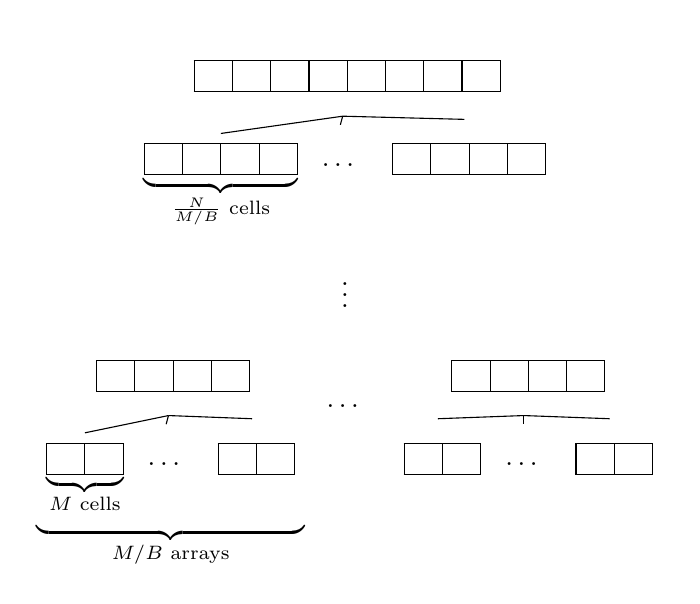
\begin{tikzpicture}[node distance=2cm and 2cm,minimum height=1cm]
  \node (A1) {
    \Tree [.{\arrayblock[& & & & & & &]{white}}
    [.{$\underbrace{\arrayblock[& & &]{white}}_{\text{$\frac{N}{M/B}$ cells}}$} ]
    [.{\ldots} ]
    [.{\arrayblock[& & &]{white}} ]
  ]  
  };
  \node[below =0mm of A1] (A2){$\vdotswithin{\ldots}$};
  \node[below left=0mm of A2] (B){
    $\underbrace{
    \Tree [.{\arrayblock[& & &]{white}}
      [.{$\underbrace{\arrayblock[&]{white}}_{\text{$M$ cells}}$} ]
      [.{\ldots} ]
      [.{\arrayblock[&]{white}} ]
    ]}_{\text{$M/B$ arrays}}$
  };
  \node[below =5mm of A2] (C){\ldots};
  \node[below right=0mm of A2] (D){
    \Tree [.{\arrayblock[& & &]{white}}
      [.{\arrayblock[&]{white}} ]
      [.{\ldots} ]
      [.{\arrayblock[&]{white}} ]
    ]
  };
\end{tikzpicture}
\end{document}
